\documentclass{article}
\usepackage{amsmath}
\usepackage{amssymb}
\usepackage{graphicx}
\usepackage{hyperref}
\usepackage[version=4]{mhchem}


\begin{document}
(2009 AMC 10 A Problem 21) Many Gothic cathedrals have windows with portions containing a ring of congruent circles that are circumscribed by a larger circle. In the figure shown, the number of smaller circles is four. What is the ratio of the sum of the areas of the four smaller circles to the area of the larger circle?\\
\centering
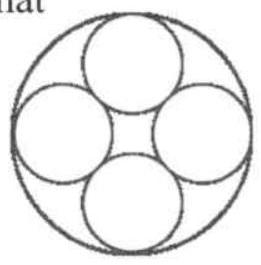
\includegraphics[width=\textwidth]{images/182(1).jpg}

Solution: \(4(3-2 \sqrt{2})\).\\
It may be assumed that the smaller circles each have radius 1 . Their centers form a square with side length 2 and diagonal length \(2 \sqrt{2}\).\\
Thus the diameter of the large circle is \(2+\sqrt{2}\), so its area is \((1+\sqrt{2})^{2} \pi=(3+2 \sqrt{2}) \pi\).\\
\centering
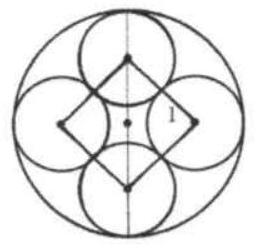
\includegraphics[width=\textwidth]{images/182(2).jpg}


The desired ratio is \(\frac{4 \pi}{(3+2 \sqrt{2}) \pi}=4(3-2 \sqrt{2})\).
\end{document}
